% =====================================================================
%  solution.tex  --  IR-SAM problem statement and contribution brief
%
%  Compile (single, self-contained pass; no external images required):
%      pdflatex solution.tex
%      pdflatex solution.tex      % second pass resolves cross-references
%  Output: solution.pdf
%
%  Dependencies: a standard TeX Live / MiKTeX installation with the
%  packages loaded below (all part of the default distribution). No
%  shell-escape, no bibliography tool, and no external graphics files
%  are needed: every figure is drawn with TikZ/pgfplots inline.
% =====================================================================
\documentclass[11pt,a4paper]{article}

\usepackage[utf8]{inputenc}
\usepackage[T1]{fontenc}
\usepackage{lmodern}
\usepackage[margin=1in]{geometry}
\usepackage{microtype}
\usepackage{amsmath,amssymb}
\usepackage{xcolor}
\usepackage{booktabs}
\usepackage{enumitem}
\usepackage{listings}
\usepackage{tikz}
\usepackage{pgfplots}
\pgfplotsset{compat=1.17}
\usetikzlibrary{arrows.meta,positioning,shapes.geometric,fit,backgrounds}
\usepackage[colorlinks=true,linkcolor=blue!55!black,citecolor=blue!55!black,
            urlcolor=blue!55!black]{hyperref}

% ---- palette -------------------------------------------------------
\definecolor{irblue}{HTML}{1F4E79}
\definecolor{irgreen}{HTML}{2E7D32}
\definecolor{irred}{HTML}{B00020}
\definecolor{irgray}{HTML}{555555}
\definecolor{irlight}{HTML}{EEF3F8}

% ---- listings ------------------------------------------------------
\lstset{
  basicstyle=\ttfamily\small,
  keywordstyle=\color{irblue}\bfseries,
  commentstyle=\color{irgray}\itshape,
  stringstyle=\color{irgreen},
  showstringspaces=false,
  columns=fullflexible,
  breaklines=true,
  frame=single,
  framesep=4pt,
  rulecolor=\color{irgray!40},
  backgroundcolor=\color{irlight},
  numbers=none,
}

\newcommand{\bottom}{\ensuremath{\bot}}
\newcommand{\irsam}{\mbox{IR\nobreakdash-SAM}}

\title{\textbf{Intent-Reconstructive Secure API Migration (\irsam)}\\[2pt]
\large A Soundness-Oriented Solution to Injection-Vulnerability Remediation}
\author{Remediation Engine --- Problem Statement and Contribution Brief}
\date{}

\begin{document}
\maketitle
\vspace{-2.2em}
\begin{center}\rule{0.85\linewidth}{0.4pt}\end{center}

\begin{abstract}
\noindent
Injection flaws (SQL, OS-command, LDAP and XPath injection) remain at the
top of industrial vulnerability inventories, yet the tooling that
\emph{detects} them has far outpaced the tooling that \emph{safely
repairs} them. Existing automated repair approaches are dominated by
machine-learning models that optimise for plausibility rather than
security and therefore offer no guarantee that an accepted patch is
actually safe. This document states the gap that \irsam{} addresses, the
motivation for a fundamentally different design point, the goal of the
work, and the novelty and contributions of the resulting system. \irsam{}
reconstructs the \emph{developer's intended} interpreter command as a
typed, hole-annotated \emph{Semantic Intent Graph}, then binds every
untrusted hole to a parameterising safe API through a verified catalog,
and refuses to act (\bottom) whenever a sound binding cannot be proven.
The design is backed by a pen-and-paper and mechanised (Lean~4) soundness
theorem and by an evaluation that shows a $0.80$ functional fix rate with
zero residual sinks, against $0.20$ and $0.15$ for representative
SAST-autofix and LLM-assisted baselines.
\end{abstract}

% =====================================================================
\section{The Gap}
% =====================================================================

Static analysis has made the \emph{discovery} of injection
vulnerabilities a largely solved engineering problem: commercial and
open-source scanners (CodeQL, Semgrep, SonarQube) routinely flag
SQL injection (CWE-89), OS-command injection (CWE-78), LDAP injection
(CWE-90) and XPath injection (CWE-643) at industrial scale. The
\emph{remediation} of those same findings, however, is still performed
by hand or delegated to tools that cannot guarantee the result is
secure. Three concrete deficiencies define the gap.

\begin{description}[leftmargin=1.4em,style=nextline]
  \item[G1 --- No soundness contract.]
  Learning-based repair systems
  (e.g.\ VulRepair~\cite{fu2022vulrepair}, SeqTrans~\cite{chi2023seqtrans},
  ChatRepair~\cite{xia2023chatrepair}, InferFix~\cite{jin2023inferfix})
  and LLM-prompted repair~\cite{pearce2023examining} produce edits that
  \emph{look} correct but carry no checkable invariant. ``Plausible'' is
  not ``safe'': a model can delete the vulnerable line, paraphrase the
  query, or introduce a half-measure escape that a determined attacker
  bypasses. There is no point in the pipeline at which the tool can be
  \emph{forced} to be right or to stay silent.

  \item[G2 --- Detector--repairer impedance mismatch.]
  Detectors emit \emph{locations}; safe repair needs \emph{intent}. A
  scanner says ``tainted data reaches \texttt{executeQuery} on line~67''.
  It says nothing about which parts of the constructed string are the
  developer's fixed query skeleton and which are the variable data that
  must be parameterised. Tools that operate purely on the host
  Abstract Syntax Tree (AST) therefore degrade to syntactic
  pattern-replacement and break on any query assembled dynamically.

  \item[G3 --- The false-fix failure mode.]
  An incorrect patch that compiles and passes a smoke test is worse than
  no patch: it closes the ticket, suppresses the scanner alert, and ships
  a still-exploitable system with a false sense of safety. No mainstream
  automated remediator treats ``I cannot prove this is safe'' as a
  first-class, auditable outcome.
\end{description}

Figure~\ref{fig:gap} situates \irsam{} against the prevailing tool
classes on the two axes that matter for production remediation:
the strength of the safety guarantee and the breadth of code shapes
handled.

\begin{figure}[t]
\centering
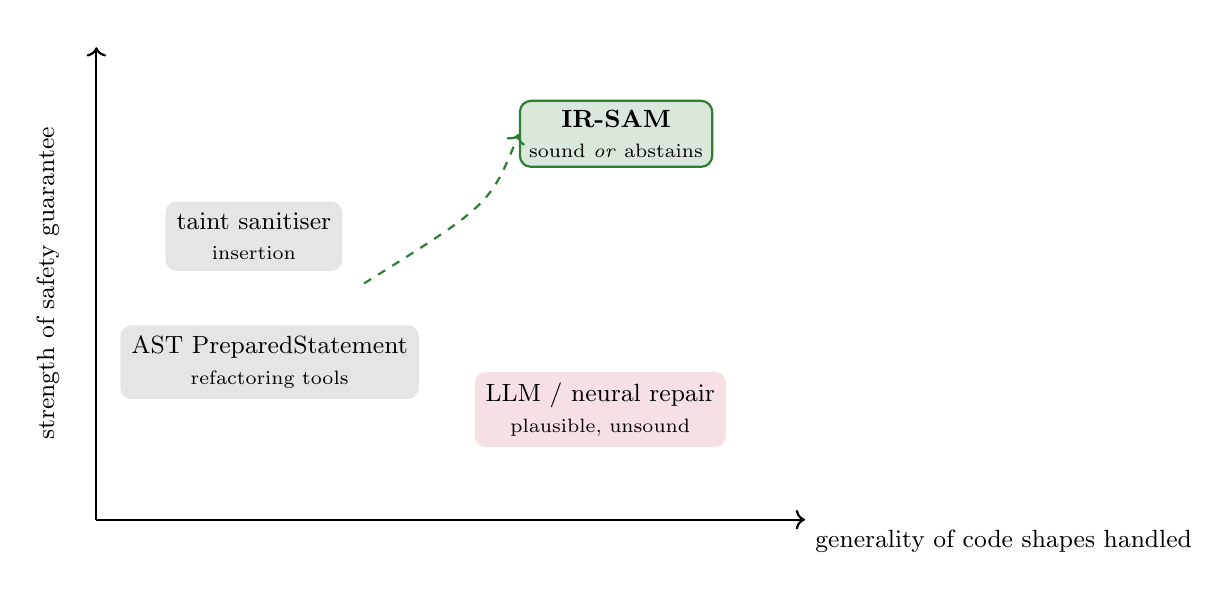
\begin{tikzpicture}[scale=1.0]
  \draw[->,thick] (0,0) -- (9,0) node[below right] {\small generality of code shapes handled};
  \draw[->,thick] (0,0) -- (0,6) node[above left] {};
  \node[rotate=90,anchor=south,font=\small] at (-0.35,3) {strength of safety guarantee};
  % regions
  \node[align=center,fill=irred!12,rounded corners,inner sep=4pt] (llm) at (6.4,1.4)
        {\small LLM / neural repair\\[-1pt]\scriptsize plausible, unsound};
  \node[align=center,fill=irgray!15,rounded corners,inner sep=4pt] (ast) at (2.2,2.0)
        {\small AST PreparedStatement\\[-1pt]\scriptsize refactoring tools};
  \node[align=center,fill=irgray!15,rounded corners,inner sep=4pt] (san) at (2.0,3.6)
        {\small taint sanitiser\\[-1pt]\scriptsize insertion};
  \node[align=center,fill=irgreen!18,rounded corners,draw=irgreen,thick] (irs) at (6.6,4.9)
        {\small \textbf{\irsam}\\[-1pt]\scriptsize sound \emph{or} abstains};
  \draw[->,irgreen,thick,dashed] (3.4,3.0) .. controls (5,4) .. (irs.west);
\end{tikzpicture}
\caption{The remediation landscape. \irsam{} targets the under-served
upper-right region: a checkable safety guarantee \emph{combined with}
coverage of dynamically constructed interpreter strings, with an explicit
abstention (\bottom) whenever soundness cannot be established.}
\label{fig:gap}
\end{figure}

% =====================================================================
\section{Motivation}
% =====================================================================

The economic and security case for closing this gap is direct.

\paragraph{Volume.} A single enterprise scan run produces thousands of
injection findings. Manual remediation does not scale; teams either defer
fixes (raising exposure) or apply rote escaping (raising the risk of an
unsound fix, G3).

\paragraph{The escaping anti-pattern is structurally weak.} Sanitisation
tries to neutralise attacker bytes \emph{inside} the interpreter's lexer
--- it keeps the data on the dangerous side of the parser and bets that
every meta-character has been escaped for every dialect. Parameterised
APIs instead move the data to the interpreter's \emph{protocol layer},
where it is never lexed as code at all. The correct fix is therefore not
``escape more carefully'' but ``relocate the data out of the grammar''.
Capturing that transformation requires understanding the \emph{intended
command}, not just the byte stream.

\paragraph{Trust requires verifiability, not plausibility.} For a
remediation tool to be deployable in a security-critical pipeline, an
auditor must be able to answer ``why is this patch safe?'' with a
structural argument, not ``a model predicted it''. This rules out
opaque generation as the final authority and motivates a design whose
acceptance criterion is a decidable structural property of the patched
code.

\paragraph{Abstention is a feature, not a failure.} Because a wrong fix
is more dangerous than an unfixed-but-flagged finding (G3), the rational
design choice is a system that \emph{prefers silence to a guess}. This
single commitment --- ``\bottom{} rather than an unsound patch'' ---
reorients the entire architecture and is the motivating principle behind
\irsam.

% =====================================================================
\section{Goal}
% =====================================================================

The goal of this work is to build and formally justify an automated
remediation engine for injection vulnerabilities that satisfies the
following requirements:

\begin{enumerate}[label=\textbf{R\arabic*.},leftmargin=2.6em]
  \item \textbf{Soundness.} Every patch the system \emph{accepts} must
  satisfy a precise, decidable soundness criterion: attacker-controlled
  data can never reach the interpreter as syntax. Formally
  (\S\ref{sec:novelty}), for an accepted patch $p$ and every host state
  $\sigma$,
  \[
    \llbracket P_I(\mathrm{exec}(p,\sigma))\rrbracket_I(\sigma)
       \in \mathrm{Intent}(A) \subseteq L_I \setminus \mathrm{Mal}_I .
  \]
  \item \textbf{Sound abstention.} When no patch can be proven sound, the
  system must return \bottom{} (with a machine-readable reason) rather
  than emit an unverified edit.
  \item \textbf{Intent fidelity.} The patched program must be observably
  equivalent to the original on benign (trusted) inputs --- the fix must
  not change what the application does for legitimate users.
  \item \textbf{Detector-agnostic operation.} The system must consume the
  output of any standard SAST tool (CodeQL, Semgrep, SonarQube) through a
  unified finding schema, so detection quality and remediation quality are
  decoupled concerns.
  \item \textbf{Multi-interpreter, multi-language reach.} The same
  pipeline must cover SQL, OS-command, LDAP and XPath sinks across Java and
  Python, with a declarative path to extend coverage.
  \item \textbf{Auditability.} Every accepted patch must carry a
  structural certificate that a reviewer (or a downstream verifier) can
  re-check independently.
\end{enumerate}

% =====================================================================
\section{Novelty \& Contribution}
\label{sec:novelty}
% =====================================================================

\irsam{} --- \emph{Intent-Reconstructive Secure API Migration} --- is, to
our knowledge, the first injection-remediation system designed around a
machine-checkable soundness contract with disciplined abstention. Its
novelty rests on four interlocking ideas.

\subsection{N1 --- Intent reconstruction instead of byte rewriting}
Rather than editing the host AST or escaping bytes, \irsam{} lifts the
dynamically constructed interpreter string into an \textbf{Intent
Abstract Model (IAM)}, a 4-tuple $A=(G,H,C,\Sigma)$:
\begin{itemize}[leftmargin=1.4em,nosep]
  \item $G$ is a typed \textbf{Semantic Intent Graph (SIG)} over the
  interpreter's grammar, with explicit \textsc{hole} nodes marking the
  positions where data flows in;
  \item $H$ annotates each hole with its grammatical role
  (\textsf{value}, \textsf{identifier}, \textsf{fragment},
  \textsf{structural}), semantic type, and cardinality;
  \item $C$ is the set of constraints (type, range, allow-list) over
  holes;
  \item $\Sigma$ is the symbol environment carrying the proof obligation
  that each identifier is a trusted constant.
\end{itemize}
This representation makes the developer's \emph{intent} --- the fixed
query skeleton versus the variable data --- a first-class, typed object
that the repair can reason about.

\subsection{N2 --- The binding function \texorpdfstring{$\varphi$}{phi}
with mandatory abstention}
A partial function $\varphi:\mathrm{IAM}\rightharpoonup\mathrm{Patch}$
maps an IAM to a host-language rewrite via a finite catalog of verified
\emph{binders}. Each binder pairs a SIG sub-pattern with a safe-API
rewrite template, checkable pre/post-conditions, and a soundness
argument. Crucially, $\varphi(A)=\bottom$ is \emph{required} whenever any
hole cannot be covered by a sound binder (e.g.\ an identifier hole whose
trust cannot be established, or grammar outside the supported fragment).
Abstention is thus part of the specification, not an error path.

\subsection{N3 --- A decidable structural soundness criterion}
We prove that a patch is IAM-sound if every \textsf{value} hole is
realised as an argument to a parameterising API call
(\texttt{PreparedStatement.setX}, \texttt{ProcessBuilder(List<String>)},
\texttt{XPathVariableResolver}, \dots) and every
\textsf{identifier}/\textsf{structural} hole is realised as an allow-list
lookup that traps on miss. This condition is \emph{decidable on the host
AST}, so the validator (pipeline stage~G) can re-check it independently of
how the patch was produced. The accompanying theorem (proved on paper for
the SQL$_0$+JDBC fragment and mechanised in Lean~4 for the identifier
closure, structural cover, audit soundness, and the main
\texttt{soundness\_parameterize} result) states that an accepted patch
admits no execution in which attacker bytes are lexed as interpreter
syntax.

\subsection{N4 --- A seven-stage, detector-agnostic pipeline}
\irsam{} is realised as the composition
$G\circ F\circ E\circ D\circ C\circ B\circ A$ shown in
Figure~\ref{fig:pipeline}: locate the sink (A), slice the
string-construction (B), reconstruct a parameterised template (C), parse
it into an IAM (D), bind via $\varphi$ (E), synthesise the host patch (F),
and validate through five independent gates (G): compilation, regression,
structural-soundness, re-SAST, and differential testing. Any SARIF-
producing detector can drive stage~A through a unified finding schema.

\begin{figure}[t]
\centering
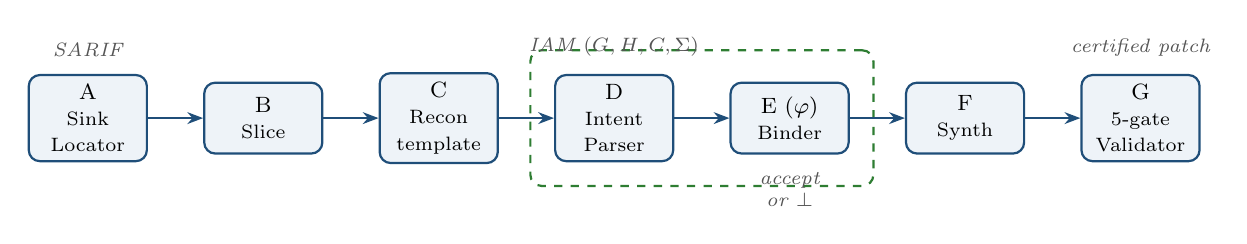
\begin{tikzpicture}[
   node distance=6.5mm and 7mm,
   stage/.style={draw=irblue,thick,fill=irlight,rounded corners,
                 minimum height=9mm,minimum width=15mm,align=center,
                 font=\footnotesize},
   io/.style={font=\scriptsize\itshape,color=irgray},
   ar/.style={-{Stealth[length=2mm]},thick,irblue}]
  \node[stage] (A) {A\\\scriptsize Sink\\\scriptsize Locator};
  \node[stage,right=of A] (B) {B\\\scriptsize Slice};
  \node[stage,right=of B] (C) {C\\\scriptsize Recon\\\scriptsize template};
  \node[stage,right=of C] (D) {D\\\scriptsize Intent\\\scriptsize Parser};
  \node[stage,right=of D] (E) {E ($\varphi$)\\\scriptsize Binder};
  \node[stage,right=of E] (F) {F\\\scriptsize Synth};
  \node[stage,right=of F] (G) {G\\\scriptsize 5-gate\\\scriptsize Validator};
  \draw[ar] (A)--(B); \draw[ar] (B)--(C); \draw[ar] (C)--(D);
  \draw[ar] (D)--(E); \draw[ar] (E)--(F); \draw[ar] (F)--(G);
  \node[io,above=1mm of A] {SARIF};
  \node[io,above=1mm of D] {IAM $(G,H,C,\Sigma)$};
  \node[io,below=1mm of E,align=center] {accept\\or \bottom};
  \node[io,above=1mm of G] {certified patch};
  \begin{scope}[on background layer]
    \node[draw=irgreen,thick,dashed,rounded corners,inner sep=3mm,
          fit=(D)(E)] {};
  \end{scope}
\end{tikzpicture}
\caption{The \irsam{} pipeline. Intent reconstruction (D) and the binding
function $\varphi$ (E) --- highlighted --- are the conceptual core; stage~G
re-checks the decidable soundness criterion of~N3 before any patch is
accepted.}
\label{fig:pipeline}
\end{figure}

\subsection{Worked example}
The transformation \irsam{} performs is illustrated below: an unsafe
concatenated JDBC query is lifted to its intent and re-emitted as a
parameterised statement that preserves behaviour on trusted inputs while
making attacker injection structurally impossible.

\begin{lstlisting}[language=Java,aboveskip=4pt,belowskip=2pt]
// BEFORE  (CWE-89: value concatenated into the SQL grammar)
String sql = "SELECT id FROM users WHERE name = '" + name + "'";
ResultSet rs = stmt.executeQuery(sql);
\end{lstlisting}
\begin{lstlisting}[language=Java,aboveskip=2pt,belowskip=4pt]
// AFTER   (value relocated to a protocol-bound parameter slot)
PreparedStatement ps =
    conn.prepareStatement("SELECT id FROM users WHERE name = ?");
ps.setString(1, name);
ResultSet rs = ps.executeQuery();
\end{lstlisting}

\subsection{Summary of contributions}
\begin{enumerate}[label=\textbf{C\arabic*.},leftmargin=2.6em]
  \item A formal intent model (IAM/SIG) and a soundness criterion for
  injection remediation that is \emph{decidable on the host AST}.
  \item A binding function $\varphi$ with a verified binder catalog and a
  specified abstention discipline that prefers \bottom{} to an unsound
  patch.
  \item A pen-and-paper and Lean~4-mechanised soundness theorem for the
  SQL$_0$+JDBC fragment, extended to OS-command (argv inertness) and path
  guards.
  \item A working, detector-agnostic, multi-interpreter
  (SQL/command/LDAP/XPath), multi-language (Java/Python) implementation
  with a five-gate validator.
  \item An empirical evaluation showing a functional fix rate of $0.80$
  with \emph{zero} residual sinks and perfect abstention precision,
  against $0.20$ (SAST-autofix) and $0.15$ (LLM-assisted) baselines,
  together with whole-repository tests on the OWASP Benchmark and other
  intentionally vulnerable projects in which \irsam{} produced
  \emph{zero unsound patches}.
\end{enumerate}

\begin{figure}[t]
\centering
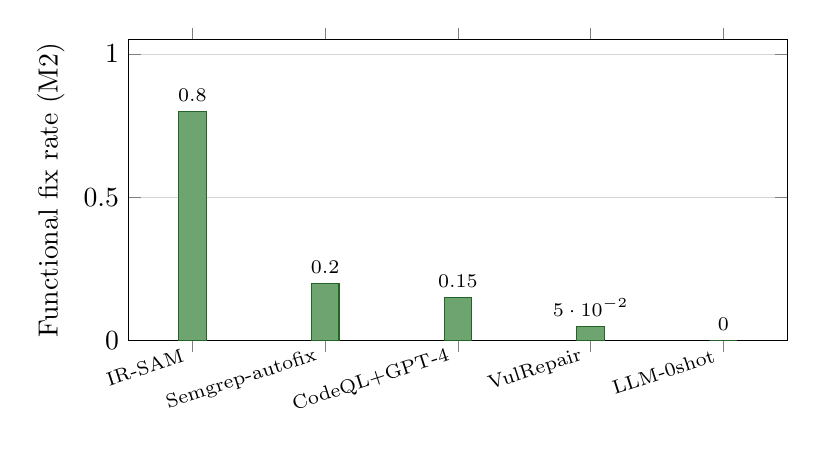
\begin{tikzpicture}
\begin{axis}[
  width=0.82\linewidth, height=5.4cm,
  ybar, bar width=10pt,
  ymin=0, ymax=1.05,
  ylabel={Functional fix rate (M2)},
  symbolic x coords={IR-SAM,Semgrep-autofix,CodeQL+GPT-4,VulRepair,LLM-0shot},
  xtick=data, x tick label style={rotate=18,anchor=east,font=\scriptsize},
  nodes near coords, nodes near coords style={font=\scriptsize},
  enlarge x limits=0.12,
  ymajorgrids, grid style={irgray!25},
]
\addplot[fill=irgreen!70,draw=irgreen!80!black] coordinates
  {(IR-SAM,0.80) (Semgrep-autofix,0.20) (CodeQL+GPT-4,0.15)
   (VulRepair,0.05) (LLM-0shot,0.00)};
\end{axis}
\end{tikzpicture}
\caption{Functional fix rate (metric M2) on the Phase-5 evaluation
($n=20$). \irsam{} fixes $4\times$ as many cases as the strongest baseline
while keeping residual sinks (M4) at zero and abstention precision (M6)
at $1.00$.}
\label{fig:m2}
\end{figure}

% =====================================================================
\section*{Conclusion}
\addcontentsline{toc}{section}{Conclusion}
% =====================================================================
The gap in injection remediation is not detection but \emph{trustworthy
repair}. \irsam{} closes it by reconstructing developer intent, binding
untrusted data to parameterising APIs through a verified catalog, and
refusing to act when soundness cannot be proven. The result is a
remediation engine whose every accepted patch carries a re-checkable
safety certificate --- and whose silence, when it occurs, is itself a
sound and auditable decision.

\bibliographystyle{plain}
\begin{thebibliography}{9}
\bibitem{fu2022vulrepair} M.~Fu, C.~Tantithamthavorn, T.~Le, V.~Nguyen,
  and D.~Phung. ``VulRepair: a T5-based Automated Software Vulnerability
  Repair.'' \emph{ESEC/FSE}, 2022.
\bibitem{chi2023seqtrans} J.~Chi et al. ``SeqTrans: Automatic
  Vulnerability Fix via Sequence to Sequence Learning.'' \emph{IEEE TSE},
  2023.
\bibitem{pearce2023examining} H.~Pearce, B.~Tan, B.~Ahmad, R.~Karri, and
  B.~Dolan-Gavitt. ``Examining Zero-Shot Vulnerability Repair with Large
  Language Models.'' \emph{IEEE S\&P}, 2023.
\bibitem{xia2023chatrepair} C.~S.~Xia and L.~Zhang. ``ChatRepair:
  Conversation-based Automated Program Repair.'' \emph{ICSE}, 2024.
\bibitem{jin2023inferfix} M.~Jin et al. ``InferFix: End-to-End Program
  Repair with LLMs.'' \emph{ESEC/FSE}, 2023.
\end{thebibliography}

\end{document}
